\chapter{Generics}
\label{chap:generics}

\fcolorbox{black}[HTML]{E9F0E9}{\parbox{\textwidth}{%
\noindent \textbf{Learning goals}\\
The junior-colleague
\begin{enumerate}[nolistsep]
\item can explain what generics is.
\item can describe type erasure and the consequences of type erasure
\item can use generic classes, methods and interfaces
\item can create generic classes, method and interfaces
\end{enumerate}}}

\begin{summary}
Java Generics provides the ability to write generic code that is independent of a data type. When a developer uses a generic class,  interface,  or method,  he will specify which data type will acutally be used. The Java Collections framework is entirely written generically. The moment you use an ArrayList,  you need to indicate the data type for the elements of your list.
\end{summary}

\section{Before generics}
Java is a strongly typed programming language.  During the compilation of a program, you will be pointed out if you use the wrong data type.

\begin{lstlisting}
Object aReference = new Movie("Brother Bear");
Integer luckyNumber = aReference;
\end{lstlisting}

The second line of code results in a compilation error.

 

When Java was introduced, this datatype check was not implemented in the Java Collections framework. The following code compiles without errors.  As soon as you execute the program, an exception will occur.

\begin{lstlisting}
import java.util.ArrayList;
import java.util.Iterator;

public class BeforeGenerics {

	public static void main(String[] args) {
		ArrayList objecten = new ArrayList();
		objecten.add(1);
		objecten.add(5.4);
		objecten.add(new Movie("Inception"));

		Iterator iterator = objecten.iterator();
		double total = 0;
		while (iterator.hasNext()) {
			total += (Double) iterator.next();
		}
		System.out.println(total);
	}
}
\end{lstlisting}


\begin{verbatim}
Exception in thread "main" java.lang.ClassCastException: class java.lang.Integer 
cannot be cast to class java.lang.Double (java.lang.Integer and java.lang.Double 
are in module java.base of loader 'bootstrap')
	at be.pxl.ja.BeforeGenerics.main(BeforeGenerics.java:24)
\end{verbatim}

Type-safety was introduced in the Java Collections framework since Java 5. 
When you open the java documentation for the class java.util.ArrayList, you will see the generic parameter  $<E>$. 
E is the type-parameter en makes it possible to provide a datatype for the elements of the ArrayList. 

\begin{lstlisting}
/**
 * Resizable-array implementation of the {@code List} interface.  Implements
 * all optional list operations, and permits all elements, including
 * {@code null}. 
 * ...
 * @param <E> the type of elements in this list
 *
 * @author  Josh Bloch
 * @author  Neal Gafter
 * @see     Collection
 * @see     List
 * @see     LinkedList
 * @see     Vector
 * @since   1.2
 */
public class ArrayList<E> extends AbstractList<E>
        implements List<E>, RandomAccess, Cloneable, java.io.Serializable {
        
    transient Object[] elementData;
    
    /**
     * Returns the element at the specified position in this list.
     *
     * @param  index index of the element to return
     * @return the element at the specified position in this list
     * @throws IndexOutOfBoundsException {@inheritDoc}
     */
    public E get(int index) {
        Objects.checkIndex(index, size);
        return elementData(index);
    }
    
    E elementData(int index) {
        return (E) elementData[index];
    }
    
    ...
}
\end{lstlisting}

\begin{lstlisting}
import java.util.ArrayList;
import java.util.Iterator;

public class SinceGenerics {

	public static void main(String[] args) {

		ArrayList<Double> objecten = new ArrayList<>();
		objecten.add((double) 1);
		objecten.add(5.4);
		//objecten.add(new Movie("Inception"));

		Iterator<Double> iterator = objecten.iterator();
		double total = 0;
		while (iterator.hasNext()) {
			total += iterator.next();
		}
		System.out.println(total);
	}
}
\end{lstlisting}

If you were to add a Movie-object to an ArrayList that accepts Double-objects, you get a compile error.

\begin{verbatim}
Error:(16, 30) java: incompatible types: be.pxl.ja.streamingservice.model.Movie 
cannot be converted to java.lang.Double
\end{verbatim}

When calling the constructor of a generic class, we use the diamond operator $<>$. The compiler can infer the datatype of the objects in the ArrayList (this is called type inference).  We don't need to repeat the datatype when calling the constructor and use the diamond operator.


\section{Writing generic classes}

The generic class Duo  contains a pair of objects of the generic datatype T.  The class definition identifies this class as a generic class by using the type parameter T (<T>).  In the Duo class, you can use T as the datatype for fields,  parameters,  and returntype.

\begin{lstlisting}
public class Duo<T> {
	private T first;
	private T second;

	public Duo(T first, T second) {
		this.first = first;
		this.second = second;
	}

	public T getFirst() {
		return first;
	}

	public T getSecond() {
		return second;
	}
}
\end{lstlisting}

At the moment you create objects of the class Duo,  you will indicate which actual datatype the type parameter T should be replaced with.  For a developer, it looks like the type parameter T is replaced by the chosen datatype.


\begin{lstlisting}
public class DifferentDuos {

	public static void main(String[] args) {
		Duo<String> cocktail = new Duo<>("gin", "tonic");
		System.out.println(cocktail.getFirst());
		Duo<Actor> famousDuo = new Duo<>(new Actor("Ben","Stiller"), new Actor("Owen", "Wilson"));
		Duo<Integer> numbers = new Duo<>(5, 12);
	}

}
\end{lstlisting}

\subsection{Naming conventions}

To avoid confusion between actual classes and generic type parameters in Java, it is important to use correct naming conventions. We will always use a single uppercase letter to name a type parameter.   According to the code conventions, you should never use a single uppercase letter as the name for a class; you must always use meaningful class names. Therefore, when you see a single uppercase letter in Java code, you may assume it is a generic parameter.

We adhere to the following guidelines:

\begin{itemize}
\item E – Element (used in the Java Collections Framework)
\item K – Key (used in Map)
\item N – Number
\item T – Type
\item V – Value (used in Map)
\item S,U,V etc. – use when T already in use
\end{itemize}

\section{Generic interfaces}

\subsection{Interface $Comparable<T>$}

The generic interface $Comparable<T>$ makes it possible to compare objects. 

Once a class implements this $Comparable<T>$ interface, you can use methods like Collections.sort(...) to sort a collection containing objects of this class. We call this ordering the natural order of the class.

When a class implements the $Comparable<T>$ interface, you fill in the type parameter T with the class itself. You must implement the method \textit{int compareTo(T e)}. Through the implementation of this method, you can compare any object of the class with another object of the same class. The int compareTo(T e) method returns:
\begin{itemize}
\item 0 if both objects are equal.
\item -1 or a negative number if this is less than the argument.
\item 1 or a positive number if this is greater than the argument.
\end{itemize}

Always try to keep the natural order of a class consistent with the implementation of equals()-method.  So, when e1.compareTo(e2) == 0, e1.equals(e2) and e2.equals(e1) should also return true.  Null does not belong to any class, so e1.compareTo(null) should always throw a NullPointerException.

\begin{figure}[H]
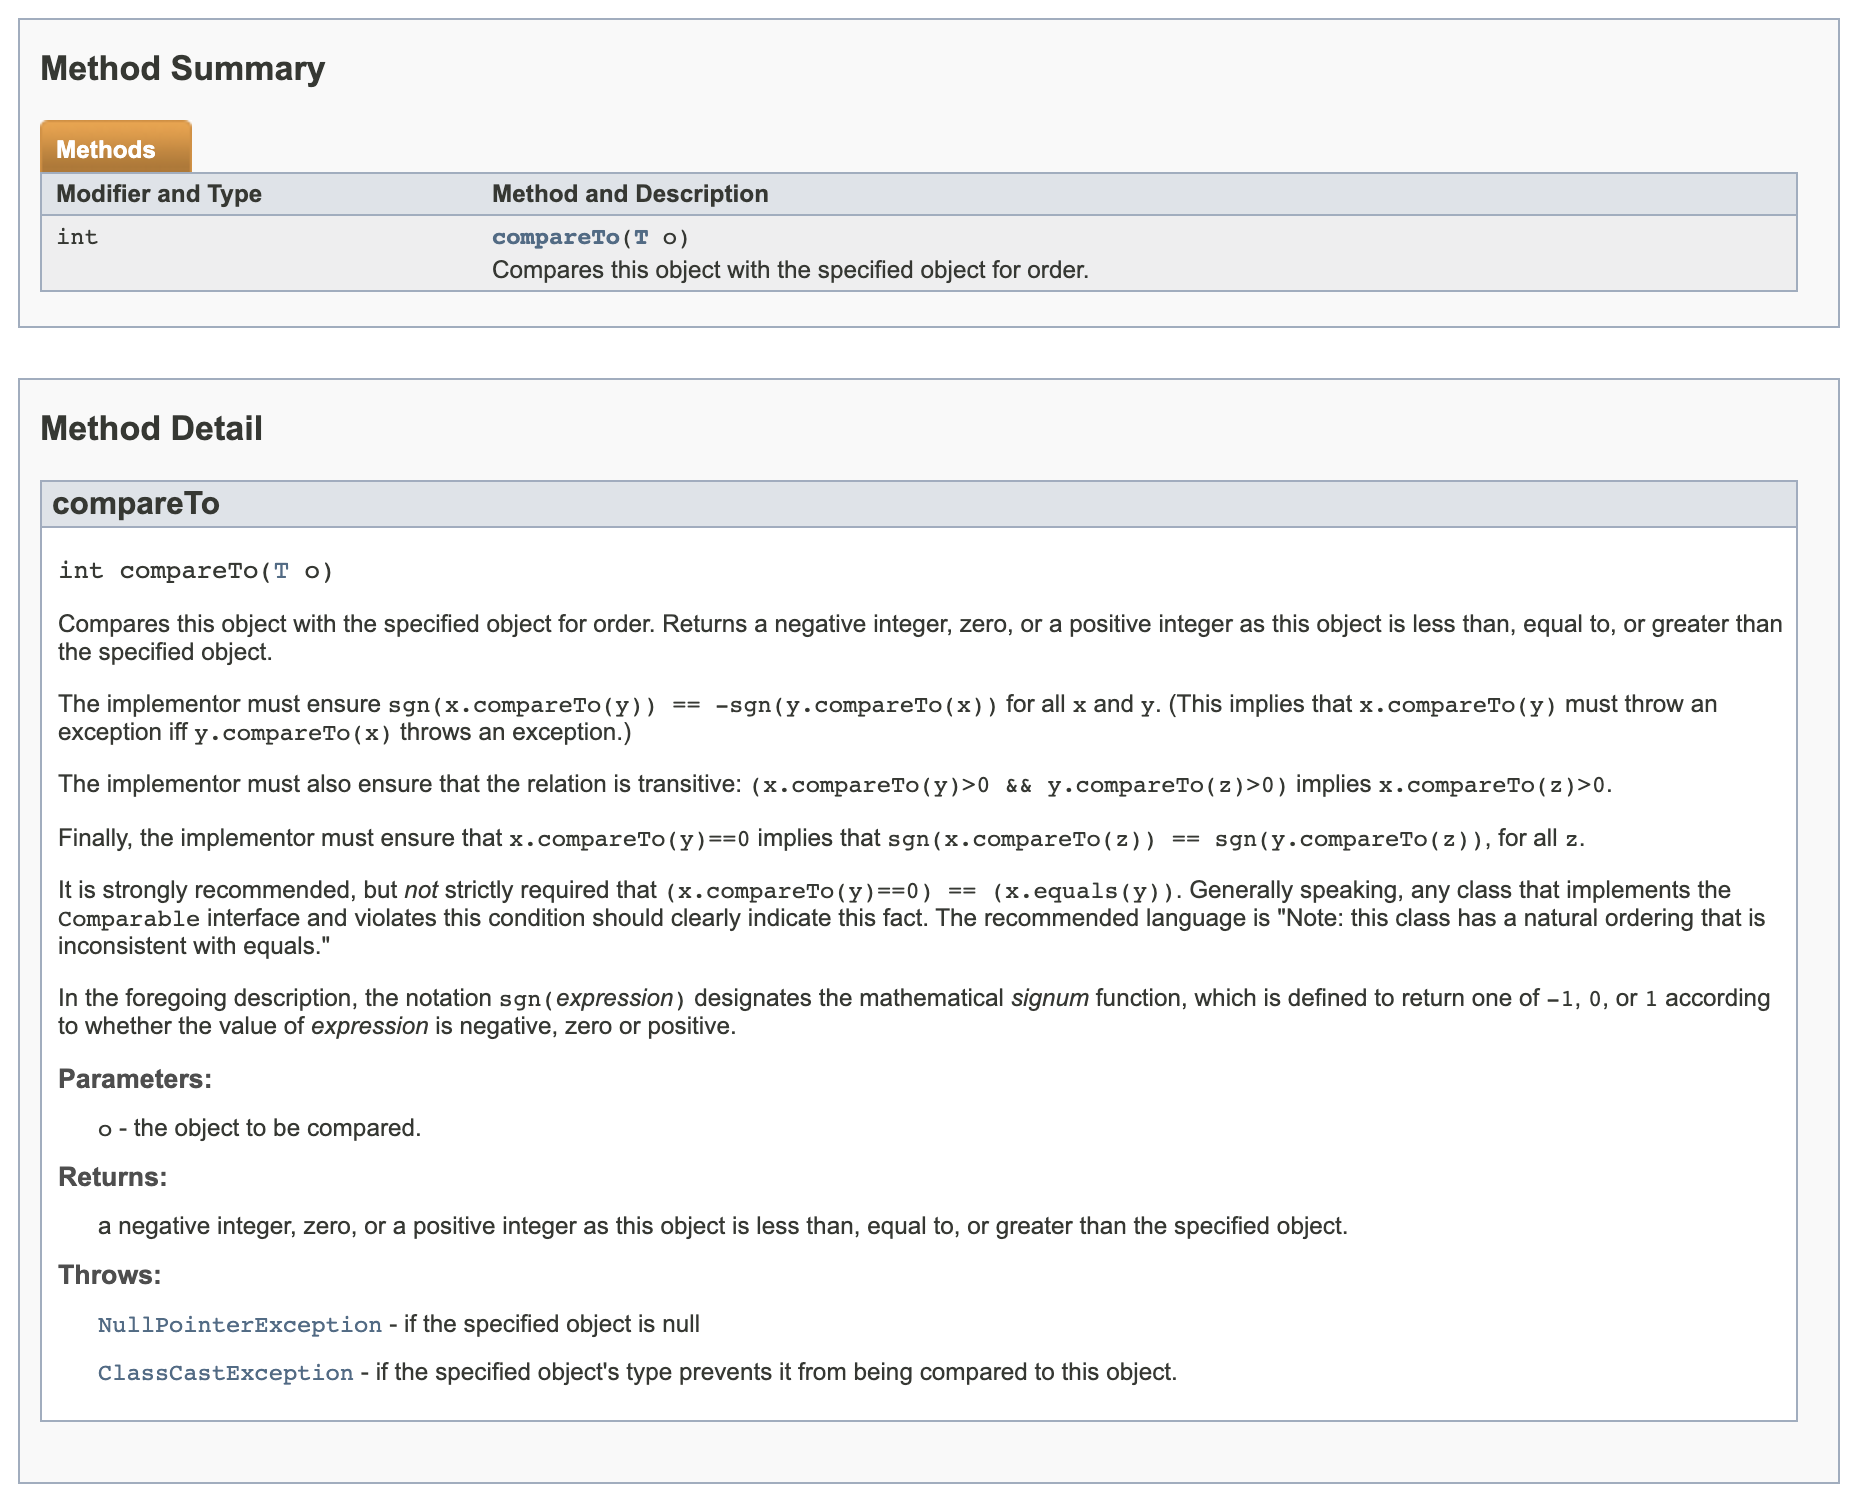
\includegraphics[width=\linewidth]{images/chapter_generics/javadoc_compareTo.png}
\caption{Documentation for interface $Comparable<T>$}
\label{fig:core_classes}
\end{figure}

The class Person has a natural ordering based on the name of a Person-object.  Objects of the class Person can be sorted alphabetically by name. When Person-objects share the same name, we sort by date of birth (younger to older).

\begin{lstlisting}
import java.time.LocalDate;
import java.time.LocalDateTime;
import java.time.temporal.ChronoUnit;
import java.util.Objects;

public class Person implements Comparable<Person> {
	private String name;
	private LocalDate dateOfBirth;

	public Person(String name, LocalDate dateOfBirth) {
		this.name = name;
		this.dateOfBirth = dateOfBirth;
	}

	public int getAge() {
		if (dateOfBirth == null) {
			return 0;
		}
		return (int) ChronoUnit.YEARS.between(dateOfBirth, LocalDateTime.now());
	}
	
	@Override
	public int compareTo(Person other) {
		int nameCompare = this.name.compareTo(other.name);
		if (nameCompare == 0) {
			return other.dateOfBirth.compareTo(this.dateOfBirth);
		}
		return nameCompare;
	}

	public String getName() {
		return name;
	}

	@Override
	public boolean equals(Object o) {
		if (this == o) {
			return true;
		}
		if (o == null || getClass() != o.getClass()) {
			return false;
		}

		Person person = (Person) o;

		if (!Objects.equals(name, person.name)) {
			return false;
		}
		return Objects.equals(dateOfBirth, person.dateOfBirth);
	}

	@Override
	public int hashCode() {
		int result = name != null ? name.hashCode() : 0;
		result = 31 * result + (dateOfBirth != null ? dateOfBirth.hashCode() : 0);
		return result;
	}

	@Override
	public String toString() {
		return "Person{" +
				"name='" + name + '\'' +
				", age='" + getAge() + '\'' +
				'}';
	}
}
\end{lstlisting}

\begin{lstlisting}
package be.pxl.demo;

import java.time.LocalDate;
import java.util.ArrayList;
import java.util.Collections;
import java.util.List;

public class SortingPersons {

	public static void main(String[] args) {
		List<Person> persons = new ArrayList<>();
		Person person1 = new Person("Erik", LocalDate.of(1998, 5, 2));
		Person person2 = new Person("Sam", LocalDate.of(2000, 5, 2));
		Person person3 = new Person("Ann", LocalDate.of(2005, 3, 1));
		Person person4 = new Person("Ann", LocalDate.of(2003, 4, 2));
		Person person5 = new Person("Ann", LocalDate.of(2003, 4, 2));

		persons.add(person1);
		persons.add(person2);
		persons.add(person3);
		persons.add(person4);
		persons.add(person5);

		System.out.println(person3.compareTo(person1));
		System.out.println(person4.compareTo(person3));
		System.out.println(person4.compareTo(person5));

		Collections.sort(persons);
		
		System.out.println(persons);
	}
}
\end{lstlisting}


\begin{verbatim}
-4
2
0
[Person{name='Ann', age='18'}, Person{name='Ann', age='20'}, Person{name='Ann', age='20'}, Person{name='Erik', age='25'}, Person{name='Sam', age='23'}]
\end{verbatim}



\subsection{Writing a generic interface}

In addition to generic classes, you can also develop generic interfaces and methods. Here is an example of a generic interface with two generic parameters T and U.

\begin{lstlisting}
public interface Service<T,U> {

	T execute(U arg);
}
\end{lstlisting}

The interface can have different parameter type and returntype, but this is not mandatory. You can, however, choose the same datatype for generic type T and U.

Als je beslist om deze interface te implementeren ben je verplicht om de methode execute te implementeren, maar je ben vrij om het datatype voor de parameter en de return-waarde te kiezen.

Hier volgen 2 klassen die de interface Service implementeren.

\begin{lstlisting}
public class CountService implements Service<Integer, String> {

	@Override
	public Integer execute(String arg) {
		return arg.length();
	}
}
\end{lstlisting}

\begin{lstlisting}
public class PersonConverterService implements Service<String, Person> {
    private static final DateTimeFormatter FORMATTER = DateTimeFormatter.ofPattern("dd/MM/yyyy");
    @Override
    public Person execute(String arg) {
        // Assuming the input format is "Name, Age"
        String[] parts = arg.split(",");
        if (parts.length != 2) {
            throw new IllegalArgumentException("Invalid input format: " + arg);
        }
        try {
            LocalDate dateOfBirth = LocalDate.parse(parts[1].trim(), FORMATTER);
            return new Person(parts[0].trim(), dateOfBirth);
        } catch (DateTimeParseException e) {
            throw new IllegalArgumentException("Invalid date format: " + arg);
        }
    }
}

public class Main {
    public static void main(String[] args) {
        Service<String, Person> personConverter = new PersonConverterService();
        Person person = personConverter.execute("John Doe, 12/03/2001");

        if (person != null) {
            System.out.println("Converted person: " + person);
        } else {
            System.out.println("Conversion failed.");
        }
    }
}
\end{lstlisting}

This program gives the following output:
\begin{verbatim}
Converted person: Person{name='John Doe', age='22'}
\end{verbatim}


\section{Generic methods}

If you don't need a fully parameterized class, it's also possible to create generic methods. Both regular and static methods can contain one or more generic types. Even a constructor can use generic parameters.

Here's an example.
The following static method \textit{occursExactTimes} returns true if the specified item occurs exactly the given number of times in the List. If not, it returns false.
Before the returntype of the method, you have to identify all the generic types that are used in the method.
 
\begin{lstlisting}
import java.util.List;

public class OccurenceUtil {

	public static <T> boolean occursExactTimes(List<T> items, T item, int times) {
		int count = 0;
		for (T anItem : items) {
			if (anItem.equals(item)) {
				count++;
			}
		}
		return count == times;
	}

}
\end{lstlisting}

The method \textit{occursExactTimes} can be used with different datatypes. 

\begin{lstlisting}
import java.util.Arrays;
import java.util.List;

public class Main {

	public static void main(String[] args) {

		List<Integer> numbers = Arrays.asList(7, 15, 23, 12, 8, 7, 23, 13, 32, 7);
		System.out.println(OccurenceUtil.occursExactTimes(numbers, 7, 3));
		System.out.println(OccurenceUtil.occursExactTimes(numbers, 23, 5));
		List<String> animals = Arrays.asList("zebra", "elephant", "kangaroo", "cow", "kangaroo");
		System.out.println(OccurenceUtil.occursExactTimes(animals, "kangaroo", 2));
	}
}
\end{lstlisting}

Executing this program will give you the following output:

\begin{verbatim}
true
false
true
\end{verbatim}



\section{Bounded generics}


Bounded means here \'restricted\', and we can restrict the datatypes that a method accepts.  Given the following class Card.

\begin{lstlisting}
public enum Suit {
	HEARTS,
	DIAMONDS,
	CLUBS,
	SPADES
}

public enum Rank {
	ACE,
	TWO,
	THREE,
	FOUR,
	FIVE,
	SIX,
	SEVEN,
	EIGHT,
	NINE,
	TEN,
	JACK,
	QUEEN,
	KING
}

public class Card implements Comparable<Card> {
    private final Suit suit;
    private final Rank rank;

    public Card(Suit suit, Rank rank) {
        this.suit = suit;
        this.rank = rank;
    }

    public Suit getSuit() {
        return suit;
    }

    public Rank getRank() {
        return rank;
    }

    @Override
    public String toString() {
        return rank + " " + suit;
    }

    @Override
    public int compareTo(Card other) {
        return this.rank.compareTo(other.rank);
    }
}
\end{lstlisting}

We have a utility class with multiple methods to find the highest value.

\begin{lstlisting}
public class MyUtil {
	static int highest(int a, int b) {
		return Math.max(a, b);
	}
	static double highest(double a, double b) {
		return Math.max(a, b);
	}
	static Card highest(Card a, Card b) {
		return a.compareTo(b) > 0 ? a : b;
	}
}

public class Main {

	public static void main(String[] args) {
		System.out.println(MyUtil.highest(5, 9));
		System.out.println(MyUtil.highest(12.6, -4.6));
		System.out.println(MyUtil.highest(new Card(Suit.HEARTS, Rank.FIVE), new Card(Suit.HEARTS, Rank.SEVEN)));
	}
}
\end{lstlisting}

This program will produce the following output:

\begin{verbatim}
9
12.6
SEVEN HEARTS
\end{verbatim}

Is it possible to write one generic method to decide on the highest value?

Let's rewrite our utility class.  Integer, Double, and Card all implement the Comparable interface. 

\begin{lstlisting}
public class MyUtil2 {

	static Integer highest(Integer a, Integer b) {
		return a.compareTo(b) > 0 ? a : b;
	}

	static Double highest(Double a, Double b) {
		return a.compareTo(b) > 0 ? a : b;
	}

	static Card highest(Card a, Card b) {
		return a.compareTo(b) > 0 ? a : b;
	}
}
\end{lstlisting}

This way we can write a generic method.  The generic method allows for comparisons of any type that implements the Comparable interface. 

\begin{lstlisting}
public class MyUtil2 {

	static <T extends Comparable<T>> T highest(T a, T b) {
		return a.compareTo(b) > 0 ? a : b;
	}
}
\end{lstlisting}


A \'bound\' or restriction is a constraint we impose on the generic type parameter.
In a bound, you can include at most 1 class; there is no restriction on the number of interfaces.  However, the class must always come first in the listing:
\textit{
$<$T extends MyClass \& MyFirstInterface \& MySecondInterface \& MyThirdInterface$>$}.

\section{Wildcards}

In generic code,  the question mark (?),  called the wildcard,  represents an unknown type.

\subsection{Unbounded wildcards}

\begin{lstlisting}
import java.util.Arrays;
import java.util.List;

public class Demo2 {

	public static void main(String[] args) {
		List<Integer> list1 = Arrays.asList(1, 2, 3);
		List<String> list2 = Arrays.asList("one", "two", "three");
		MyUtil.printList(list1);
		MyUtil.printList(list2);
	}
}
\end{lstlisting}

How can you write a generic method to display the elements of a list. 
If you think the following method will do the job, feel free to try:

\begin{lstlisting}
import java.util.List;

public class MyUtil {

	public static void printList(List<Object> list) {
		for (Object element: list) {
			System.out.print(element + " ");
		}
		System.out.println();
	}
}
\end{lstlisting}

However, this wil give a compilation error.

\begin{verbatim}
incompatible types: java.util.List<java.lang.Integer> cannot be converted to java.util.List<java.lang.Object>

Required type: List<Object>
Provided: List<Integer>
\end{verbatim}

Using an unbounded wildcard will do the job. 
\begin{lstlisting}
import java.util.List;

public class MyUtil {

	public static void printList(List<?> list) {
		for (Object element: list) {
			System.out.print(element + " ");
		}
		System.out.println();
	}
}
\end{lstlisting}

Occasionally,  a generic type parameter can be replaced with a wildcard. 
As shown in the example below, secondFunction will give a compile error.  Essentially, as a rule of thumb, you may read data with an unknown data type (thus a wildcard), but you may not write the data.

\begin{lstlisting}
public class Experiment {
    public static <E> void firstFunction(List<E> list) {
        list.add(list.get(0));
    }

    public static void secondFunction(List<?> list) {
        list.add(list.get(0)); // !!!!!!!!!!!!!! won't compile !!!!!!!!!
    }
}
\end{lstlisting}

\subsection{Upper bound wildcards}

\begin{lstlisting}
public static void process(List<? extends Foo> list) { /* ... */ }
\end{lstlisting}

The upper bounded wildcard matches Foo and any subtype of Foo.

\subsection{Lower bound wildcards}


Say you want to write a method that puts Integer objects into a list. To maximize flexibility, you would like the method to work on List<Integer>, List<Number>, and List<Object> — anything that can hold Integer values.

\begin{lstlisting}
public static void addNumbers(List<? super Integer> list) {
    for (int i = 1; i <= 10; i++) {
        list.add(i);
    }
}
\end{lstlisting}


\section{Type Erasure and consequences}

Generics exist only \textbf{at compile time}. During the compilation of Java code,  various additional checks are performed on generic classes to ensure the correct use of data types. Then, when generating the bytecode, all information about the generic data type is simply removed. So,  List<T> is, after some checks and the addition of extra code by the compiler, replaced by List<Object> and List<T extends Person> becomes List<Person>. This is what we call type erasure.  In Java, there will always be only one compiled class (.class file) generated for a generic class.

\begin{lstlisting}
List<Integer> list1 = new ArrayList<>();
List<Float> list2 = new ArrayList<>();
if (list1.getClass() == list2.getClass()) {
	System.out.println("Lists have same class.");
}
\end{lstlisting}

Due to type erasure, it is not possible to create generic static variables in a class. It is also not possible to call a constructor of a generic data type. Furthermore, it is not possible to use the generic data type with the instanceof operator.

\begin{lstlisting}
class Box<T> {
   //compiler error
   private static T value;
   private T t;
   
   public Box() {
      // compiler error
   	  t = new T();
   }

   public void set(T t) {
      this.t = t;
   }

   public T get() {
      return t;
   } 
   
   public boolean test() {
       // compile error
	  return t instanceof T;
   }  
}
\end{lstlisting}

\begin{remark}
More information can be found on pluralsight: \url{https://app.pluralsight.com/player?course=java-generics}. 
\end{remark}


\section{Exercise}

\begin{oefening}
Create an abstract class Player with a member variable name. Provide a constructor with  parameter name
\\
Create 3 subclasses for this abstract class Player: BaseballPlayer, VolleyballPlayer, and SoccerPlayer.
\\
Now create a class Team with the following properties:
\\
\begin{itemize}
\item name (String)
\item played (number of games played)
\item won (number of games won)
\item lost (number of games lost)
\item tied (number of games drawn)
\item members (collection of players)
\end{itemize}

Provide getters.  In the constructor,  you pass the name for the team.
\\

Provide a method \textit{addPlayer} to add a player to the team and a method \textit{numberOfPlayers} to ask for the number of players in the team.
\\
Can you add players of a different type (e.g., BaseballPlayer and SoccerPlayer) to one team? Test it! Make sure this is no longer possible.
\\
Provide the method \textit{matchResult(Team opponent, int ourScore, int theirScore)}. This method ensures that for the team for which the method is called and the opponent, the number of played, won, lost, and drawn matches is increased depending on the values for ourScore and theirScore.
\\
Can you call this method (matchResult) for a team of volleyball players against a team of baseball players? Solve this if necessary, so that this is no longer possible.
\\
Finally, add a method \textit{ranking()}. This returns an integer where the team gets 3 points for each win and 1 point for a draw. Now make sure you can create a collection of Team objects and sort them based on the ranking.
\end{oefening}



